%----------------------------------------------------------------------------------------
%	PACKAGES AND DOCUMENT CONFIGURATIONS
%----------------------------------------------------------------------------------------
% Wersja: 06.11.2017
\documentclass{article}

\usepackage[T1]{fontenc}
\usepackage{siunitx} % Provides the \SI{}{} and \si{} command for typesetting SI units
\usepackage{graphicx} % Required for the inclusion of images
\usepackage[nottoc]{tocbibind} % bibliografia
%\usepackage{natbib} % Required to change bibliography style to APA
\usepackage{amsmath} % Required for some math elements 
\setlength\parindent{12pt} % Removes all indentation from paragraphs
%\usepackage{times} % Uncomment to use the Times New Roman font

\usepackage[export]{adjustbox}

\usepackage[utf8]{inputenc} % Język polski
\usepackage{polski}
\usepackage[polish]{babel}

\usepackage[top=1in, bottom=1.25in, left=1.25in, right=1.25in]{geometry} % Marginesy
\usepackage{listings} % Kod programu
\usepackage{indentfirst} % Wcięcie przy pomocy \par
\usepackage{multicol} % Kilka kolumn dla itemize
\usepackage[table,xcdraw]{xcolor} % Dla tabel
\usepackage{float} % Blokowanie tabeli przed przemieszczeniem
%\usepackage{karnaugh-map} % Karnaugh

%\renewcommand{\labelenumi}{\alph{enumi}.} % Zamienia litery w enumerate na a, b, c, ...

%----------------------------------------------------------------------------------------
%	DOCUMENT INFORMATION
%----------------------------------------------------------------------------------------

\title{UCiSW 2 \\ \textit{Odtwarzacz .wav}} % Title

%\author{name \textsc{name}} % Author name

\date{23.05.2018} % Date for the report
%\date{\today} % Date for the report

\begin{document}

\maketitle % Insert the title, author and date

\begin{center}
\begin{tabular}{l r}
Informacja: & XX  \\ % Date the experiment was performed 
%Prowadzący: & Mgr inż. Jan Paweł II % Instructor/supervisor
Prowadzący: & Dr inż. Jarosław Sugier
\end{tabular}
\end{center}

\tableofcontents % Spis treści

% If you wish to include an abstract, uncomment the lines below
% \begin{abstract}
% Abstract text
% \end{abstract}

%----------------------------------------------------------------------------------------
%	SECTION 0
%----------------------------------------------------------------------------------------

%\begin{multicols}{2}
%	\begin{itemize}
%		\item 
%	\end{itemize}
%\end{multicols}

%\newpage
%\section{Tytuł}} 
%\subsection{Tytuł}
%\par Tekst

%\begin{itemize}
%	\item\textit{Tekst} - opis
%\end{itemize}

%\begin{enumerate}
%	\item Opis
%\end{enumerate}

%\begin{center}
%	\includegraphics[scale=0.6, center]{nazwa_pliku}
%\end{center}

%\begin{lstlisting}[basicstyle=\small]
%	kod programu;
%\end{lstlisting}

%----------------------------------------------------------------------------------------
%	SECTION 1
%----------------------------------------------------------------------------------------
\newpage
\section{Wprowadzenie}
\subsection{Cel projektu}
\par Celem projektu było stworzenie programu wczytującego plik .wav z karty pamięci, pobranie metadanych i odtworzenie dźwięku.
\subsection{Sprzęt}
\begin{itemize}
	\item{Spartan-3E (XC3S500E)}
	\item{Karta SD}
	\item{Głośnik}
\end{itemize}

\subsection{Teoria}
\par 
%----------------------------------------------------------------------------------------
%	SECTION 2
%----------------------------------------------------------------------------------------
\newpage
\section{Projekt}
\subsection{Schemat oraz wykorzystane moduły}
\begin{center}
	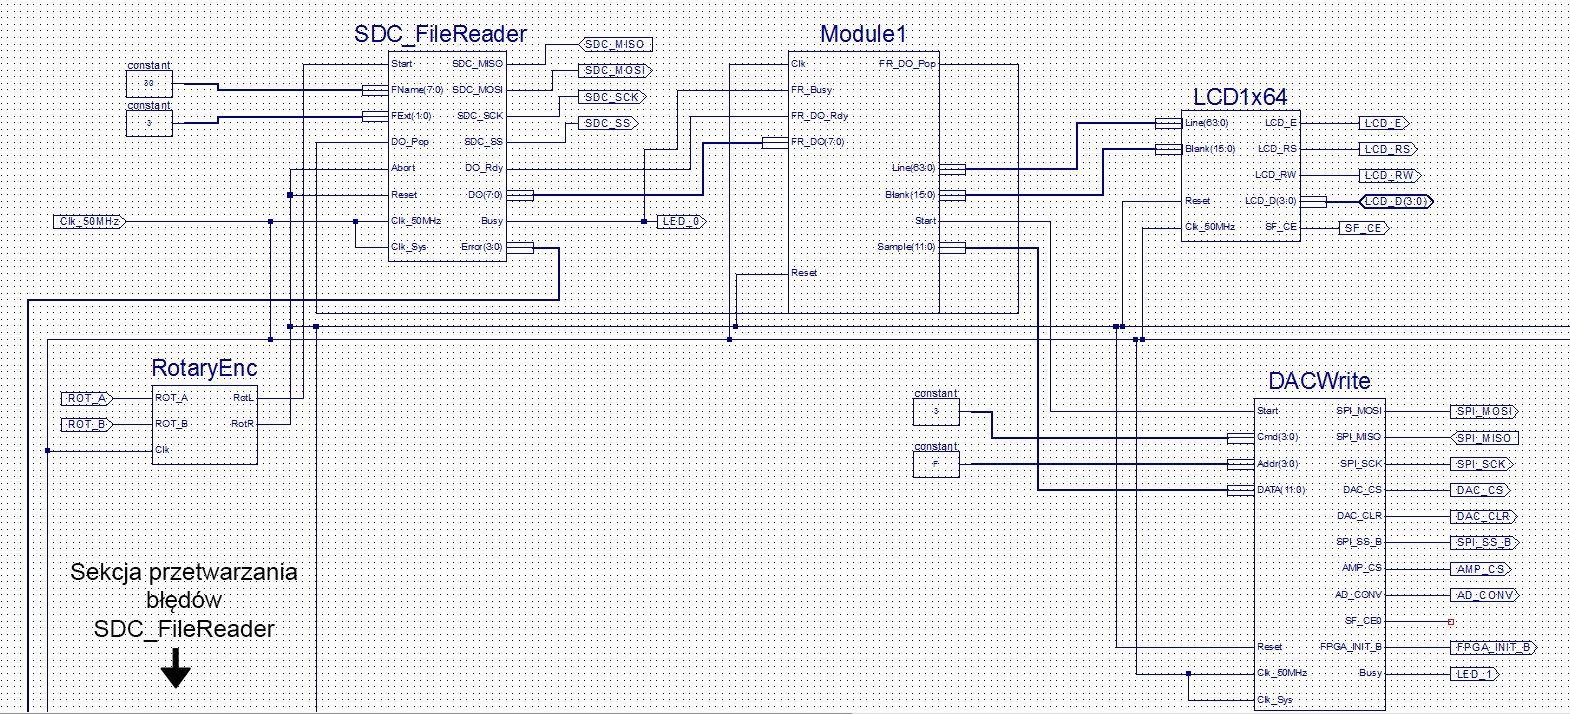
\includegraphics[scale=0.5, center]{photo/sch_horizontal.png}
\end{center}
\par Wykorzystane moduły pochodzące ze strony zsk.ict.pwr.wroc.pl/zsk\_ftp/fpga:
\begin{itemize}
	\item{RotaryEnc}: Pozwala na użycie enkodera przyrostowego
		\subitem{Obrót w lewo}: Start (SDC\_FileReader)
		\subitem{Obrót w prawo}: Reset (wszystkie moduły)
	\item{SDC\_FileReader} Pozwala odczytywać dane z karty SD
		\subitem W projekcie odczytuje on pliki .wav ("11" => FExt)
		\subitem Nazwa pliku: kod ASCII => FName
	\item{LCD1x64}: Wyświetla dane na ekranie Spartan 3E - w tym przypadku metadane pliku .wav
	\item{DACWrite}: Wysyła dane do przetwornika DAC
		\subitem Sygnał pojawia się na wszystkich pinach ("1111" => Addr)
		\subitem Sygnał wysyłany jest natychmiastowo ("0011" => Cmd)
\end{itemize}

\newpage
\subsection{Moduł Module1}
\par Moduł ten ma za zadanie odpowiednio sterować SDC\_FileReader by pobrać bajty metadanych oraz dźwięku z pliku .wav. Moduł musi również wysyłać próbki dźwięku w odpowiedniej częstotliwośći do DACWrite.
\subsubsection{WE/WY}
\begin{lstlisting}[basicstyle=\small]
Port ( 
	Clk : in STD_LOGIC;
	Reset: in STD_LOGIC;
	-- Komunikacja z SDC_FileReader
	FR_Busy : in  STD_LOGIC;
	FR_DO : in  STD_LOGIC_VECTOR (7 downto 0);
	FR_DO_Rdy : in  STD_LOGIC;
	FR_DO_Pop : out  STD_LOGIC;
	-- Zawartosc wyswietlacza 
	Line : out STD_LOGIC_VECTOR (63 downto 0) := (others => '0');
	Blank : out STD_LOGIC_VECTOR (15 downto 0);
	-- Probka oraz sygnal startu odczytu dla DACWrite
	Sample : out STD_LOGIC_VECTOR (11 downto 0) := (others => '0');
	Start : out STD_LOGIC);
\end{lstlisting}

\subsubsection{Sygnały}
\begin{lstlisting}[basicstyle=\small]
signal state, nextState : stateType;
-- Licznik odczytanych bajtow
signal counter : signed (63 downto 0) := (others => '0');
-- Licznik dlugosci przerwy miedzy wysylaniem probek
signal counterSampleRate : unsigned (15 downto 0) := (others => '0');
-- Metadane
signal numChannels : STD_LOGIC_VECTOR (15 downto 0);
signal sampleRate : STD_LOGIC_VECTOR (31 downto 0);
signal bitsPerSample : STD_LOGIC_VECTOR (15 downto 0);
\end{lstlisting}

\subsubsection{Proces 1 - przejście między stanami}
\par Proces również wykrywa sygnał Reset - przechodzi wtedy do odpowiedniego stanu (Q0R).
\begin{lstlisting}[basicstyle=\small]
process1 : process (Clk, state, Reset)
begin
	if Reset = '1' then
		state <= Q0R;
	elsif rising_edge(Clk) then
		state <= nextState;
	end if;
end process process1;
\end{lstlisting}

\newpage
\subsubsection{Proces 2 - wybór następnego stanu}
\begin{lstlisting}[basicstyle=\small]
process2 : process(state, FR_DO, FR_DO_Rdy, FR_Busy, counter, counterSampleRate)
begin
	nextState <= state;
	case state is
	
	when Q0 =>
		if FR_Busy = '1' then
			nextState <= Q1;
		else
			nextState <= Q0;
		end if;
		
	when Q0R =>
		nextState <= Q0;
\end{lstlisting}
\par Stan Q0 trwa do momentu pobudzenia modułu SDC\_FileReader przez jednotaktowy sygnał z enkodera - sygnał FR\_Busy o wartości 1 wskazuje na to że moduł SDC\_FileReader pracuje.
\par Stan Q0R to stan Reset.
\begin{lstlisting}[basicstyle=\small]
	when Q1 =>
		if FR_DO_Rdy = '1' then              
			nextState <= Q2;
		else
			nextState <= Q1;
		end if;
\end{lstlisting}
\par Stan Q1 oczekuje na bajt - SDC\_FileReader sygnalizuje koniec ładowania bajtu przy pomocy sygnału FR\_DO\_Rdy o wartości 1. 
%\newpage
\par Pobieranie metadanych wygląda następująco:
\begin{lstlisting}[basicstyle=\small]
process3: process(Clk, state, FR_DO_Rdy, FR_DO)
	begin
	if rising_edge(Clk) and state = Q1 and FR_DO_Rdy = '1' then
		if counter = X"16" then
			numChannels(7 downto 0) <= FR_DO;
			Line(7 downto 0) <= FR_DO;
		elsif counter = X"17" then
			numChannels(15 downto 8) <= FR_DO;
			Line(15 downto 8) <= FR_DO;
		elsif counter = X"18" then
			sampleRate(7 downto 0) <= FR_DO;
			Line(23 downto 16) <= FR_DO;
		elsif counter = X"19" then
			sampleRate(15 downto 8) <= FR_DO;
			Line(31 downto 24) <= FR_DO;
		elsif counter = X"1A" then
			sampleRate(23 downto 16) <= FR_DO;
			Line(39 downto 32) <= FR_DO;
		elsif counter = X"1B" then
			sampleRate(31 downto 24) <= FR_DO;
			Line(47 downto 40) <= FR_DO;
		elsif counter = X"22" then
			bitsPerSample(7 downto 0) <= FR_DO;
			Line(55 downto 48) <= FR_DO;
		elsif counter = X"23" then
			bitsPerSample(15 downto 8) <= FR_DO;
			Line(63 downto 56) <= FR_DO;
		end if;
	end if;
end process process3; 
\end{lstlisting}
\par Program sprawdza obecnie wczytywany bajt - jeżeli jest to jeden z bajtów zawierających interesujące nas metadane, zostaje przekazany do odpowiedniego sygnału.

\begin{lstlisting}[basicstyle=\small]     
	when Q2 =>      
		if counter >= X"4D" then
			nextState <= Q3;
		else
			nextState <= Q1;
		end if;
\end{lstlisting}
\par Stan Q2 sprawdza obecnie wczytywany bajt - jeżeli wczytano wszystkie bajty metadanych (bajty do 77) program przechodzi do dalszych stanów odpowiedzialnych za wczytywanie bajtów dźwięku; w innym przypadku następuje powrót do Q1.
\begin{lstlisting}[basicstyle=\small]      
	when Q3 => 
		if FR_DO_Rdy = '1' then              
			nextState <= Q4;
		else
			nextState <= Q3;
		end if;
\end{lstlisting}
\par Stan Q3 działa analogicznie do Q1 - oczekuje na bajt.
\par Pobieranie dźwięku wygląda następująco:
\begin{lstlisting}[basicstyle=\small]
process4: process(Clk, state, FR_DO_Rdy, FR_DO)
	begin
	if rising_edge(Clk) and state = Q3 and FR_DO_Rdy = '1' then
		sample(11 downto 4) <= FR_DO;
	end if;
end process process4;
\end{lstlisting}
\par Przed stanem Q3 występuje stan Q3B który nadaje odpowiednie tempo odczytywania (oraz w konsekwencji - wysyłania) dźwięku. Odpowiedni sygnał jest inkrementowany oraz sprawdzany - gdy przekroczy odpowiednią wartość stan Q3B przechodzi do Q3.
\par Ze względu na brak czasu projekt jest przystosowany pod pliki .wav o częstotliwości 8000 KHz - wartość ta powinna być porównywana z sygnałem sampleRate umożliwiając różne wartości odczytane z metadanych.
\begin{lstlisting}[basicstyle=\small]
when Q3B =>
	if counterSampleRate >= X"186A" then          
		nextState <= Q3;
	else 
		nextState <= Q3B;
end if;
\end{lstlisting}
\par Proces odpowiedzialny za inkrementacje oraz zerowanie sygnału counterSampleRate:

\begin{lstlisting}[basicstyle=\small]
 process4b: process(Clk, state, counterSampleRate)
	begin 
	if rising_edge(Clk) then
		if state = Q3B then
			counterSampleRate <= counterSampleRate + 1;
		elsif state = Q4 then
			counterSampleRate <= X"0000";
		end if;
	end if;
end process process4b;
\end{lstlisting}
\newpage
\begin{lstlisting}[basicstyle=\small]
	when Q4 =>
		if FR_Busy = '0' then
			nextState <= Q5;
		else
			nextState <= Q3B;
		end if;
\end{lstlisting}
\par Stan Q4 weryfikuje to czy SDC\_FileReader pracuje - FR\_Busy o wartości 0 sygnalizuje że wszystkie bajty zostały odczytane; program przechodzi wtedy do stanu końcowego Q5. W przeciwnym przypadku następuje powrót do odczytywania bajtów w Q3 (przez Q3B).
\par W stanie Q4 następuje również zawiadomienie modułu DACWrite tak by ten rozpoczął ładowanie przesłanej próbki:
\begin{lstlisting}[basicstyle=\small]
Start <= '1' when state = Q4
	else '0';
\end{lstlisting}
\par Ostatnim stanem jest Q5 - pętla końcowa:
\begin{lstlisting}[basicstyle=\small]
	when Q5 =>
		nextState <= Q5;
	
	end case;
end process process2;
\end{lstlisting}
\newpage 
\subsubsection{Diagram stanów}
\begin{center}
	
\includegraphics[scale=0.5, center]{photo/states.png}
\end{center}

\subsection{Symulacja}
%----------------------------------------------------------------------------------------
%	SECTION 3
%----------------------------------------------------------------------------------------
\newpage
\section{Implementacja}
%----------------------------------------------------------------------------------------
%	SECTION 4
%----------------------------------------------------------------------------------------
\newpage
\section{Podsumowanie}
\subsection{Ocena krytyczna}

\subsection{Wnioski}
\par TEST \cite{ug230} \cite{wave} \cite{zsk} test
%----------------------------------------------------------------------------------------
%	BIBLIOGRAPHY
%----------------------------------------------------------------------------------------
\newpage
\bibliographystyle{abbrv}
\bibliography{ucisw_bib}


%----------------------------------------------------------------------------------------
\end{document}